\section{Threading made easy: OpenMP}

\begin{frame}{Threads}
	\begin{itemize}
		\item Reminder: a thread is an independent sequence of instructions that can be managed by a scheduler. Multiple threads can exist for one process, with shared memory. May induce \textbf{race conditions} (e.g., data race).
		\item Using dedicated libraries (e.g., pthreads) may be cumbersome, especially since, in scientific computing, the paradigm is usually different.\begin{center}
			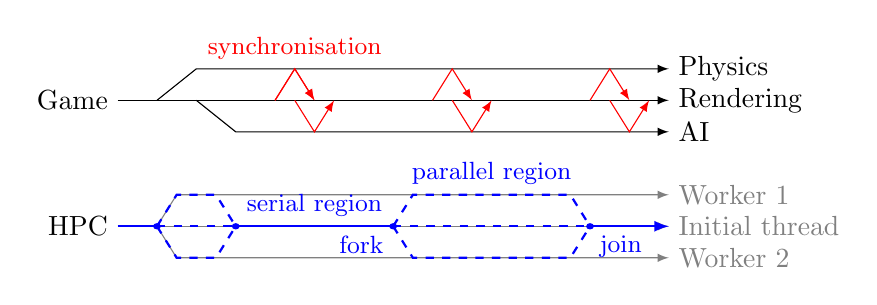
\begin{tikzpicture}[yscale=.8]
				\draw[-latex] (0,0) node[left]{Game} -- +(7,0) node[right]{Rendering};
				\draw[-latex] (.5, 0) -- ++(.5,.5) --  ++(6,0)node[right]{Physics};
				\draw[-latex] (1, 0) -- ++(.5,-.5) --  ++(5.5,0) node[right]{AI};
				\draw [red, -latex] (2,0) -- ++(.25,.5) -- ++(.25,-.5);
				\draw [red, -latex] (2,0) -- ++(.25,.5) node[above]{\small synchronisation} -- ++(.25,-.5);
				\draw [red, -latex] (2.25,0) -- ++(.25,-.5) -- ++(.25,.5);
				\draw [red, -latex] (4,0) -- ++(.25,.5) -- ++(.25,-.5);
				\draw [red, -latex] (4.25,0) -- ++(.25,-.5) -- ++(.25,.5);
				\draw [red, -latex] (6,0) -- ++(.25,.5) -- ++(.25,-.5);
				\draw [red, -latex] (6.25,0) -- ++(.25,-.5) -- ++(.25,.5);
				\begin{scope}[yshift=-2cm]
					\draw[-latex,gray] (0,0) node[left,black]{HPC} -- +(7,0) node[right]{Initial thread};
					\draw[-latex,gray] (.5, 0) -- ++(.25,.5) --  ++(6.25,0)node[right]{Worker 1};
					\draw[-latex,gray] (.5, 0) -- ++(.25,-.5) --  ++(6.25,0)node[right]{Worker 2};
					
					\draw[blue,thick] (0,0) -- ++(.5,0);
					\fill[blue] (.5,0) circle (.05cm);
					\draw[blue,dashed,thick] (.5,0) -- ++(.25,.5) -- ++(.5,0) -- ++(.25,-.5);
					\draw[blue,dashed,thick] (.5,0) -- ++(1,0);
					\draw[blue,dashed,thick] (.5,0) -- ++(.25,-.5) -- ++(.5,0) -- ++(.25,.5);
					\fill[blue] (1.5,0) circle (.05cm);
					\draw[blue,thick] (1.5,0) -- ++(2,0) node[midway,above]{\small serial region};
					\fill[blue] (3.5,0) circle (.05cm) node[anchor=north east]{\small fork};
					\draw[blue,dashed,thick] (3.5,0) -- ++(.25,.5) -- ++(2,0) node[midway,above]{\small parallel region} -- ++(.25,-.5);
					\draw[blue,dashed,thick] (3.5,0) -- ++(2.5,0);
					\draw[blue,dashed,thick] (3.5,0) -- ++(.25,-.5) -- ++(2,0) -- ++(.25,.5);
					\fill[blue] (6,0) circle (.05cm) node[anchor=north west]{\small join};
					\draw[blue,-latex,thick] (6,0) -- ++(1,0);
				\end{scope}
			\end{tikzpicture}
		\end{center}
		\item OpenMP is built on the fork/join paradigm, and generally does not use synchronization.
	\end{itemize}
\end{frame}

\begin{frame}[fragile]{OpenMP}
	\begin{itemize}
		\item Main paradigm in scientific computing for single-node applications!
		\item To use OpenMP, add directives (\cdx{\#pragma omp}) and rely on the compiler for the underlying details. One of the advantages is that it allows an \textbf{incremental} adoption.
		\item But, of course, there are still two problems that the compiler cannot solve on its own: \begin{enumerate}
			\item data dependencies:\begin{ccode}
for(i=2;i<N;i++) // Vietnam flashback, anyone?
	a[i] = a[i-1] + a[i-2];
			\end{ccode}
			\item data race (more on that later):\begin{ccode}
int x = 0;
for(i=0;i<N;i++)
	x = x + a[i];
			\end{ccode}
		\end{enumerate}
	\end{itemize}
\end{frame}

\begin{frame}[fragile]{Hello, world!}
	\begin{ccode}
#include <stdio.h>
#include <omp.h>

int main() {
	#pragma omp parallel
	{ // fork!
		printf("I'm thread %d of %d\n",
			omp_get_thread_num(), omp_get_num_threads());
	} // implicit join
}
	\end{ccode}
	Compile and execute:
	\begin{textcode}
$ gcc -o hello hello.c -fopenmp
$ OMP_NUM_THREADS=4 ./hello
I'm thread 0 of 4
I'm thread 2 of 4
I'm thread 3 of 4
I'm thread 1 of 4
	\end{textcode}
\end{frame}

\begin{frame}[fragile]{Parallel $\neq$ Worksharing }
	\begin{itemize}
		\item The content of the parallel region is executed by all threads:\begin{ccode}
#pragma omp parallel
{
	for(i=0;i<N;i++)
		a[i] = a[i]+ 1;
} // each thread execute the N iterations
		\end{ccode}
		\item Explicit work sharing:\begin{ccode}
#pragma omp parallel
{
	int t = omp_get_thread_num();
	int n = omp_get_num_threads();
	int low = N * t / n, high = N * (t + 1) / n;
	for(int i = low; i < high; i++)
		a[i] = a[i] + 1;
} // each thread do its part
		\end{ccode}
	\end{itemize}
\end{frame}

\begin{frame}[fragile]{Parallel $\neq$ Worksharing}
	But there is an easier way:
	\begin{itemize}
		\item With a directive...\begin{ccode}
#pragma omp parallel
{
	#pragma omp for
	for(i=0;i<N;i++)
		a[i] = a[i]+ 1;
} // each thread do its part
		\end{ccode}
		\item ... And directives can be combined:\begin{ccode}
#pragma omp parallel for
for(i=0;i<N;i++)
	a[i] = a[i]+ 1; // no curly braces required, but barrier
		\end{ccode}
	\end{itemize}
	Note: of course, \cdx{\#pragma omp for} must be in a parallel region (otherwise, it is only bound to the master thread). It may be useful for \textbf{orphaning}, though.
\end{frame}

\begin{frame}[fragile]{Say hello to data race!}
	\begin{ccode}
#include <stdio.h>
#include <omp.h>

int main() {
	int i, n; // ... why not?
	#pragma omp parallel
	{
		i = omp_get_thread_num(); n = omp_get_num_threads();
		printf("I'm thread %d of %d\n", i, n);
	}
}
	\end{ccode}
	Compile and execute gives (sometimes\footnote{Data race is difficult to spot, since they do not happen every time ;)}):
	\begin{textcode}
$ OMP_NUM_THREADS=4 ./hello
I'm thread 2 of 4
I'm thread 2 of 4
I'm thread 3 of 4
I'm thread 2 of 4
	\end{textcode}
\end{frame}

\begin{frame}[fragile]{First problem: communism. Let's privatize!}
	\begin{itemize}
		\item Any variable declared outside a parallel region is shared by default.
		\item Either we declare them inside:\begin{ccode}
#pragma omp parallel
{
	int i = omp_get_thread_num(); // private
	int n = omp_get_num_threads(); // private
	printf("I'm thread %d of %d\n", i, n);
}
		\end{ccode}
		\item Or we use the \cdx{private(list)} clause:\begin{ccode}
int i, n;
#pragma omp parallel private(i,n)
{
	i = omp_get_thread_num();
	n = omp_get_num_threads();
	printf("I'm thread %d of %d\n", i, n);
}
		\end{ccode}
	\end{itemize}
\end{frame}

\begin{frame}[fragile]{Privatization issue: initial value}
	\begin{ccode}
int i = 1;
#pragma omp parallel private(i)
printf("Value is %d\n", i + 1);
	\end{ccode}
	gives\begin{textcode}
$ OMP_NUM_THREADS=1 ./tmp
Value is 1
	\end{textcode}
	Why? Because private variables are \textbf{not} initialized by default in the parallel region. You should use \cdx{firstprivate}, which initialize to its value in the main thread, for that:\begin{ccode}
i = 1;
#pragma omp parallel firstprivate(i)
printf("Value is %d\n", i + 1);
	\end{ccode}
	which gives\begin{textcode}
$ OMP_NUM_THREADS=1 ./tmp
Value is 2
	\end{textcode}
\end{frame}

\begin{frame}[fragile]{Second problem: communism IS usefull!}
	\begin{ccode}
int sum = 0;
#pragma omp parallel for
for (int i=0; i < N; i++)
	sum += a[i]; // numbers from 1 to 8
printf("Sum is %d\n", sum);
	\end{ccode}
	This gives (sometimes!):\begin{textcode}
$ OMP_NUM_THREADS=1 ./tmp
Sum is 36
$ OMP_NUM_THREADS=2 ./tmp
Sum is 26
	\end{textcode}
	The problem is, again, data race. But using \cdx{private(sum)} will not help, since we want the overall result.
\end{frame}

\begin{frame}[fragile]{The solution: reduction}
	The solution is the \cdx{reduction(op:list)} clause.
	\cdx{op} is a reduction operator, which can be either arithmetic (\cdx{+ - * max min}) or logical (\cdx{\& \&\& | ||}).
	
	\begin{ccode}
#pragma omp parallel for reduction(+:sum)
for (int i=0; i < N; i++)
	sum += a[i]; // will compute a private sum
// then, it will `op` (here, add) the results of all threads
	\end{ccode}
	Could have been written with a critical\footnote{Equivalent to a mutex} or atomic region instead:\begin{ccode}
#pragma omp parallel for
for (int i=0; i < N; i++) {
	#pragma omp atomic
	sum += a[i];
}
	\end{ccode}
... But you get an overhead due to synchronization!
\end{frame}

\begin{frame}{Loop scheduling}
	\begin{itemize}
		\item The \cdx{schedule(kind[,size])} clause specifies how iterations are divided into contiguous chunks (of a given \cdx{size}), and how these chunks are distributed to the threads. \cdx{kind} may be
		\begin{itemize}
			\item \cdx{static} (default), iterations are divided into chunks, assigned to the threads. Each chunks contains the same number of iterations, except the last one.
			\item \cdx{dynamic}, the chunks are requested then processed by the thread. Implies a little \textbf{overhead}.
			\item \cdx{guided}, similar to \cdx{dynamic}, but the size of the chuncks depends on the number of remaining iteration.
		\end{itemize}
		\item The two last are usefull when the runtime of an iteration is not constant in time: equal sharing of iteration $\neq$ equal workload.
	\end{itemize}
	
	\begin{center}
		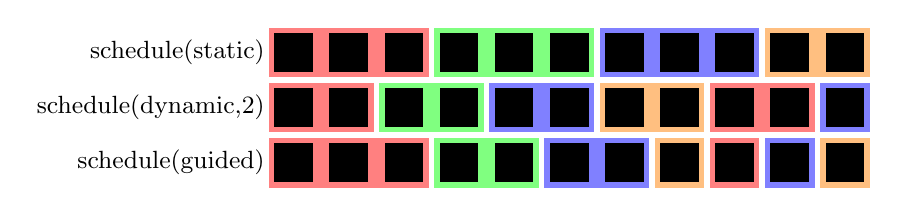
\begin{tikzpicture}[scale=.7]
			\draw (0,.35) node[left]{\small \cdx{schedule(static)}};
			\fill[red!50] (-.1,-.1) rectangle +(2.9,.9);
			\fill[green!50] (2.9,-.1) rectangle +(2.9,.9);
			\fill[blue!50] (5.9,-.1) rectangle +(2.9,.9);
			\fill[orange!50] (8.9,-.1) rectangle +(1.9,.9);
			\draw (0,-.65) node[left]{\small \cdx{schedule(dynamic,2)}};
			\fill[red!50] (-.1,-1.1) rectangle +(1.9,.9);
			\fill[green!50] (1.9,-1.1) rectangle +(1.9,.9);
			\fill[blue!50] (3.9,-1.1) rectangle +(1.9,.9);
			\fill[orange!50] (5.9,-1.1) rectangle +(1.9,.9);
			\fill[red!50] (7.9,-1.1) rectangle +(1.9,.9);
			\fill[blue!50] (9.9,-1.1) rectangle +(.9,.9);
			
			\draw (0,-1.65) node[left]{\small \cdx{schedule(guided)}};
			\fill[red!50] (-.1,-2.1) rectangle +(2.9,.9);
			\fill[green!50] (2.9,-2.1) rectangle +(1.9,.9);
			\fill[blue!50] (4.9,-2.1) rectangle +(1.9,.9);
			\fill[orange!50] (6.9,-2.1) rectangle +(.9,.9);
			\fill[red!50] (7.9,-2.1) rectangle +(.9,.9);
			\fill[green!50] (8.9,-2.1) rectangle +(.9,.9);
			\fill[blue!50] (8.9,-2.1) rectangle +(.9,.9);
			\fill[orange!50] (9.9,-2.1) rectangle +(.9,.9);
			\foreach \i in {0,1,...,10} {
				\fill (\i,0) rectangle +(.7, .7);
				\fill (\i,-1) rectangle +(.7, .7);
				\fill (\i,-2) rectangle +(.7, .7);
			}
		\end{tikzpicture}
	\end{center}
\end{frame}

\begin{frame}[fragile]{Example: number of prime numbers}
	Computing $\pi(n)$, i.e., the number of primes less than or equals to $n$:
	\begin{ccode}
int n = 100000, not_prime = 2;
#pragma omp parallel for reduction(+:not_prime)
for(int i=2; i < n; i++) {
	for (int j=2; j < i; j++) { // large `i` requires more...
		if (i % j == 0) {
			not_prime++;
			break; // ... But iteration may be very short!
		}
	}
}
printf("Pi(%d) = %d\n", n, n - not_prime);
\end{ccode}
Here, scheduling is clearly interesting (but once again, the compiler cannot know that in advance)
\end{frame}

\begin{frame}[fragile]{Example: number of prime numbers}


\begin{textcode}
$ OMP_NUM_THREADS=4 ./pi
                      default     static    dynamic     guided
      n      pi(n)       time       time       time       time
--------------------------------------------------------------
  65536       6542    0.38501    0.34878    0.21439    0.21869
 131072      12251    1.37137    1.46954    0.82317    0.81649
 262144      23000    4.95654    5.70368    3.97412    3.98117
 524288      43390   19.36867   19.65254   13.46914   12.13314
1048576      82025   73.35597   76.84343   44.77434   44.33497
\end{textcode}
As expected, clear advantage of \cdx{dynamic} and \cdx{guided} over \cdx{static}.
\end{frame}

%\begin{frame}[fragile]{FYI: explicit synchronization}
%	\begin{table}
%		\begin{tabular}{lp{8cm}}
%			\toprule
%			Directive & Result \\
%			\midrule
%			\mintinline{c}{barrier} & Explicit wait point for all threads\\
%			\mintinline{c}{master} & Block of instruction only executed by the master thread\\
%			\mintinline{c}{single} & Block of instruction only executed by one of the thread\\
%			\mintinline{c}{critical} & Critical region, only one thread can execute it at the time. May be named.\\
%			\mintinline{c}{atomic} & Limited to a few operations. Sometimes supported by hardware.\\
%			\bottomrule
%		\end{tabular}
%	\end{table}
%\begin{ccode}
%#pragma omp parallel firstprivate(local_sum)
%{
%	#pragma omp for
%	for(i=0;i<n;i++) { // note: barrier even w/o `{`!
%		local_sum += a[i];
%	} // implicit barrier here, probably not usefull
%	#pragma omp atomic
%	sum += local_sum;
%} // implicit barrier
%\end{ccode}
%One can use \mintinline{c}{#pragma omp for nowait} to lift the barrier.
%\end{frame}

\begin{frame}{Results (\cdx{*axpy})}
\begin{figure}
	\centering
	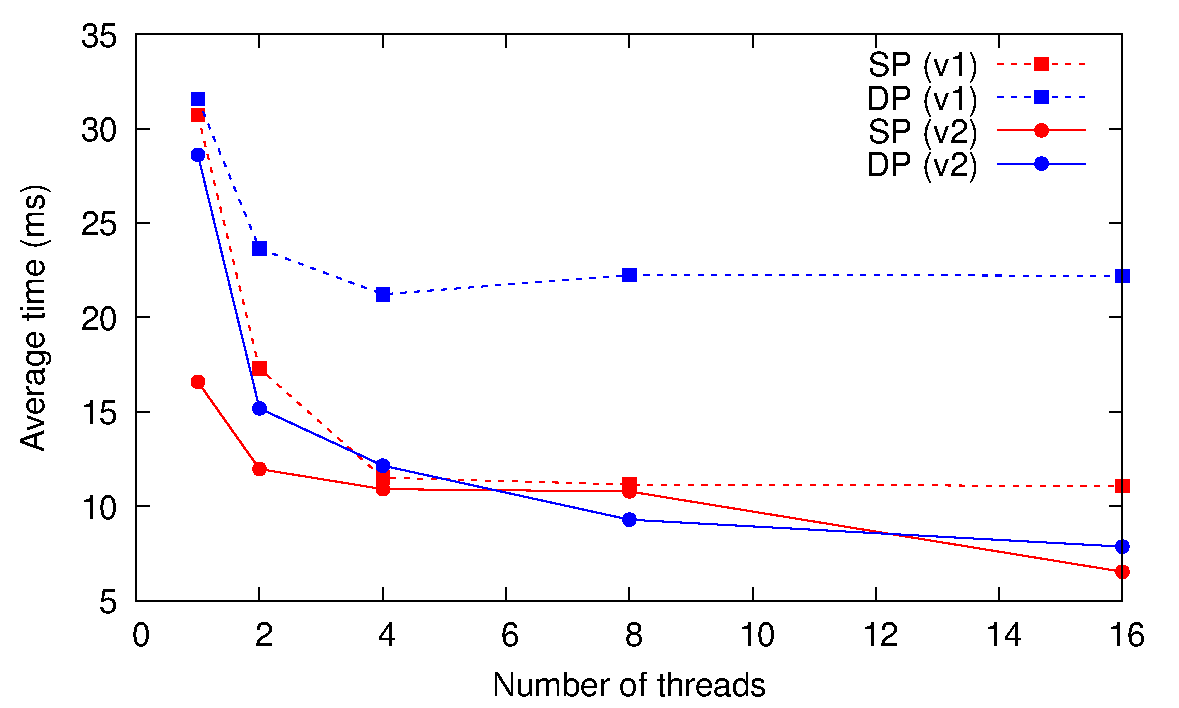
\includegraphics[width=.75\textwidth]{im/result_OMP_saxpy}
	\caption{Results for \cdx{*axpy} ($2^{24}$ numbers) with \cdx{-N 1000} and different values of \cdx{OMP\_NUM\_THREADS}.}
\end{figure}
\begin{itemize}
	\item SP faster than DP.
	\item Modest improvement for 8 and 16 threads (memory bandwidth).
	\item Second version adds SIMD and ``first touch''.
\end{itemize}
\end{frame}

\begin{frame}{Results (\cdx{*dot})}
	\begin{figure}
		\centering
		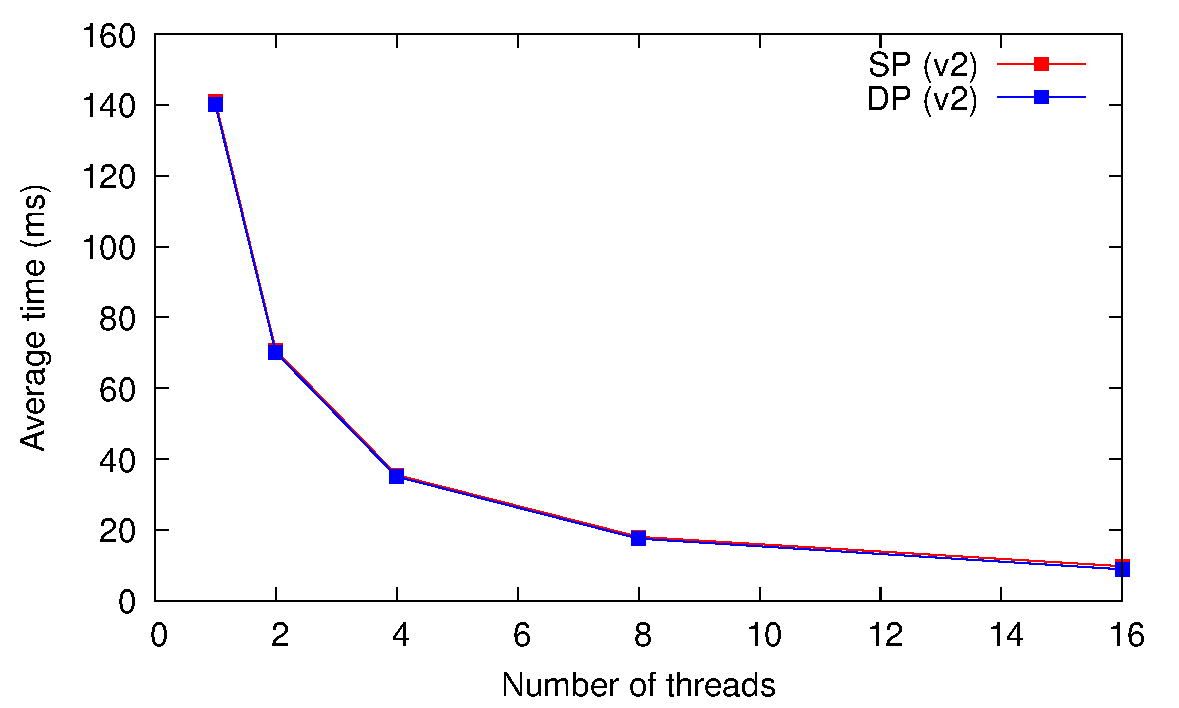
\includegraphics[width=.75\textwidth]{im/result_OMP_dot}
		\caption{Results for \cdx{*dot} ($2^{24}$ numbers) with \cdx{-N 1000} and different values of \cdx{OMP\_NUM\_THREADS}.}
	\end{figure}
\begin{itemize}
	\item Not much difference between SP and DP.
	\item More work intensive loops $\rightarrow$ better speedup with a large number of threads.
\end{itemize}
\end{frame}

\begin{frame}{Going further}
	\begin{itemize}
		\item Explicit synchronization (e.g., \cdx{critical}) ;
		\item Tasks (OpenMP 3.0) for better scheduling: allow parallelizing \cdx{while} loops and recursive call. 
		\item Thread and memory management (NUMA, thread affinity, etc).
	\end{itemize}
\end{frame}